\documentclass[11pt,a4paper]{article}
\usepackage[margin=2.2cm]{geometry}
\usepackage{booktabs,graphicx,amsmath,xcolor,float,caption}
\usepackage[T1]{fontenc}
\usepackage{lmodern}
\graphicspath{{fig/}}
\newcommand{\DataState}{prelim, 2026-11-27 12:17}
\newcommand{\DataNote}{\textbf{Preliminary.} 10 finished runs (of 25 planned), 4 jobs still queued or running at 2026-11-27 12:17.}
   % defines \DataState and \DataNote (written by prelim.sh)
\title{ALF node throughput at $\beta=L$: GPU node vs CPU node\\\large SuperMUC-NG Phase 2, test of 2026-11-27}
\author{}
\date{\DataState}
\begin{document}
\maketitle
\begin{center}\fcolorbox{red}{white}{\parbox{0.9\textwidth}{\DataNote}}\end{center}

\section{What is compared}
One full Phase 2 node per simulation: either its two CPUs alone (112 cores, build \texttt{build\_cpu-pp}, ALF 410c7b04)
or its four Intel Data Center GPU Max 1550 (8 tiles) with ALF 410c7b04 (\texttt{build\_pp}) and with the Intel-optimised
production binary (branch intel-batched, d1060305, run-time switches of the production run RUN\_L36\_batched).
Hubbard model, square lattice, $L\in\{16,24,32,36\}$, $\beta=L$ (160 to 360 time slices), $\Delta\tau=0.1$, $h_0=0$, $U=5.25$, $M_z=$ F,
Symm and Checkerboard on, Ltau $=0$, submatrix updates with $N_\text{delay}=64$, Nwrap $=10$.
Each run does NBin sweeps (NSweep $=1$): NBin $=6$ (5 timed), for the CPU at $L=32,36$ NBin $=3$ or 4 (2 or 3 timed); the first sweep is dropped. Only the configurations that were best at $\beta=4$ are run: CPU \texttt{t1}, \texttt{t2} (and \texttt{t4} at $L=36$ as backup; \texttt{t1} at $L=36$ was killed by signal 9 after 14 min without a finished sweep, most likely out of memory: about 4\,GB of stored decompositions per process, $\approx 435$\,GB for 112 processes, so \texttt{t2} is the best possible CPU configuration at $L=36$), ALF GPU \texttt{w2t7}, \texttt{w4t3}, Intel-optimised \texttt{w4t1}, \texttt{w4t3}.
All walkers of a run form one parameter set; one bin is the average of one sweep over all walkers.

\section{Node and layouts (x axes of the figures)}
Node: 2 sockets $\times$ 56 cores (Xeon Platinum 8480L), 2 NUMA domains (cores 0--55 and 56--111). GPUs 0, 1 are
attached to NUMA domain 0, GPUs 2, 3 to NUMA domain 1, so each tile has 14 nearby cores. No rank crosses a NUMA domain.

\begin{table}[H]\centering\small
\caption{CPU layouts. Tag \texttt{t}$T$ = $T$ OpenMP threads per MPI rank (one walker per rank), ranks split evenly over
the two sockets, each rank pinned to $T$ consecutive physical cores of one socket.}
\begin{tabular}{@{}llrrrr@{}}\toprule
tag & commit & threads per rank & ranks (walkers) & ranks per socket & cores used\\\midrule
\texttt{t1} & \texttt{410c7b04} & 1 & 112 & 56 & 112\\
\texttt{t2} & \texttt{410c7b04} & 2 & 56 & 28 & 112\\
\texttt{t4} & \texttt{410c7b04} & 4 & 28 & 14 & 112\\
\texttt{t6} & \texttt{410c7b04} & 6 & 18 & 9 & 108\\
\texttt{t8} & \texttt{410c7b04} & 8 & 14 & 7 & 112\\\bottomrule
\end{tabular}\end{table}

\begin{table}[H]\centering\small
\caption{GPU layouts (both GPU binaries). Tag \texttt{w}$W$\texttt{t}$T$ = $W$ walkers (MPI ranks) per tile on all 8 tiles,
$T$ OpenMP host threads per rank. Each rank is bound to the 14 cores next to its tile; compute engines per tile set with
\texttt{ZEX\_NUMBER\_OF\_CCS}. \texttt{w4t3} is the production layout; \texttt{w4t1} checks whether host threads matter.}
\resizebox{\textwidth}{!}{\begin{tabular}{@{}llrrrr@{}}\toprule
tag & commits & walkers per tile & ranks (walkers) & threads per rank & compute engines per tile\\\midrule
\texttt{w1t14} & \texttt{410c7b04}, \texttt{d1060305} & 1 & 8 & 14 & 1\\
\texttt{w2t7} & \texttt{410c7b04}, \texttt{d1060305} & 2 & 16 & 7 & 2\\
\texttt{w4t3} & \texttt{410c7b04}, \texttt{d1060305} & 4 & 32 & 3 & 4\\
\texttt{w8t1} & \texttt{410c7b04}, \texttt{d1060305} & 8 & 64 & 1 & 4\\
\texttt{w4t1} & \texttt{410c7b04}, \texttt{d1060305} & 4 & 32 & 1 & 4\\\bottomrule
\end{tabular}}\end{table}

\section{Timing and throughput}
Rank 0 writes one bin per sweep to \texttt{data.h5}, one HDF5 write per observable. The modification time of the file is
logged with ns resolution; the writes form 12 bursts (file creation + 11 bins). For the timed sweeps $k=2,\dots,11$:
\[
t_\text{comp}(k)=\text{first write of bin }k-\text{last write of bin }k{-}1,\qquad
t_\text{io}(k)=\text{last write of bin }k-\text{first write of bin }k .
\]
Production writes one bin per 10 sweeps, so the cost per sweep is $t_\text{sweep}=t_\text{comp}+t_\text{io}/10$.
Walkers synchronise at every bin, so $t_\text{sweep}$ is the time of the slowest walker. With $N_w$ walkers on the node,
\[
\text{throughput}=\frac{3600\,N_w}{\bar t_\text{sweep}}\ \text{sweeps per node-hour},\qquad
\sigma=\text{throughput}\cdot\frac{\sigma_{\bar t}}{\bar t},
\]
with $\sigma_{\bar t}$ the standard error of the timed sweeps.

Energy per sweep (estimate from vendor TDP, to be checked): CPU-only node $2\times350$\,W $=700$\,W,
GPU node $4\times600$\,W $+700$\,W $=3100$\,W; $E=P_\text{node}\cdot3600/\text{throughput}$.

\section{Results}
\begin{table}[h]\centering\small
\caption{Best layout per side: node throughput (sweeps per node-hour) and factor against the best CPU layout.}\label{tab:summary}
\begin{tabular}{@{}rllllr@{}}\toprule
$L$ & side & commit & best layout & sweeps per node-hour & factor vs CPU\\\midrule
16 & CPU & \texttt{410c7b04} & -- & running & --\\
16 & GPU & \texttt{410c7b04} & \texttt{w4t3} & $25\,602 \pm 76$ & --\\
16 & GPU Intel-opt. & \texttt{d1060305} & -- & running & --\\
\addlinespace
24 & CPU & \texttt{410c7b04} & -- & running & --\\
24 & GPU & \texttt{410c7b04} & \texttt{w4t3} & $4\,679 \pm 10$ & --\\
24 & GPU Intel-opt. & \texttt{d1060305} & -- & running & --\\
\addlinespace
32 & CPU & \texttt{410c7b04} & -- & running & --\\
32 & GPU & \texttt{410c7b04} & \texttt{w2t7} & $1\,431 \pm 3$ & --\\
32 & GPU Intel-opt. & \texttt{d1060305} & \texttt{w4t1} & $3\,652 \pm 2$ & --\\
\addlinespace
36 & CPU & \texttt{410c7b04} & -- & running & --\\
36 & GPU & \texttt{410c7b04} & \texttt{w2t7} & $814 \pm 2$ & --\\
36 & GPU Intel-opt. & \texttt{d1060305} & -- & running & --\\
\bottomrule\end{tabular}\end{table}
\begin{table}[h]\centering\small
\caption{All layouts at $L=16$ ($\beta=4$). Time per sweep of one walker (mean of the timed sweeps, $\pm$ standard error; averaged over repeats) and node throughput.}
\begin{tabular}{@{}llllrr@{}}\toprule
side & commit & tag & layout & time per sweep (s) & sweeps per node-hour\\\midrule
GPU & \texttt{410c7b04} & \texttt{w2t7} & 2 walker/tile, 7 thr. & $2.527 \pm 0.005$ & $22\,789 \pm 48$\\
GPU & \texttt{410c7b04} & \texttt{w4t3} & 4 walker/tile, 3 thr. & $4.500 \pm 0.013$ & $25\,602 \pm 76$\\
\bottomrule\end{tabular}\end{table}
\begin{table}[h]\centering\small
\caption{All layouts at $L=24$ ($\beta=4$). Time per sweep of one walker (mean of the timed sweeps, $\pm$ standard error; averaged over repeats) and node throughput.}
\begin{tabular}{@{}llllrr@{}}\toprule
side & commit & tag & layout & time per sweep (s) & sweeps per node-hour\\\midrule
GPU & \texttt{410c7b04} & \texttt{w2t7} & 2 walker/tile, 7 thr. & $12.408 \pm 0.101$ & $4\,642 \pm 38$\\
GPU & \texttt{410c7b04} & \texttt{w4t3} & 4 walker/tile, 3 thr. & $24.619 \pm 0.053$ & $4\,679 \pm 10$\\
\bottomrule\end{tabular}\end{table}
\begin{table}[h]\centering\small
\caption{All layouts at $L=32$ ($\beta=4$). Time per sweep of one walker (mean of the timed sweeps, $\pm$ standard error; averaged over repeats) and node throughput.}
\begin{tabular}{@{}llllrr@{}}\toprule
side & commit & tag & layout & time per sweep (s) & sweeps per node-hour\\\midrule
GPU & \texttt{410c7b04} & \texttt{w2t7} & 2 walker/tile, 7 thr. & $40.255 \pm 0.089$ & $1\,431 \pm 3$\\
GPU & \texttt{410c7b04} & \texttt{w4t3} & 4 walker/tile, 3 thr. & $88.303 \pm 0.065$ & $1\,305 \pm 1$\\
GPU Intel-opt. & \texttt{d1060305} & \texttt{w4t1} & 4 walker/tile, 1 thr. & $31.541 \pm 0.018$ & $3\,652 \pm 2$\\
GPU Intel-opt. & \texttt{d1060305} & \texttt{w4t3} & 4 walker/tile, 3 thr. & $34.467 \pm 0.070$ & $3\,342 \pm 7$\\
\bottomrule\end{tabular}\end{table}
\begin{table}[h]\centering\small
\caption{All layouts at $L=36$ ($\beta=4$). Time per sweep of one walker (mean of the timed sweeps, $\pm$ standard error; averaged over repeats) and node throughput.}
\begin{tabular}{@{}llllrr@{}}\toprule
side & commit & tag & layout & time per sweep (s) & sweeps per node-hour\\\midrule
GPU & \texttt{410c7b04} & \texttt{w2t7} & 2 walker/tile, 7 thr. & $70.766 \pm 0.144$ & $814 \pm 2$\\
GPU & \texttt{410c7b04} & \texttt{w4t3} & 4 walker/tile, 3 thr. & $155.706 \pm 0.080$ & $740 \pm 0$\\
\bottomrule\end{tabular}\end{table}


\begin{figure}[H]\centering
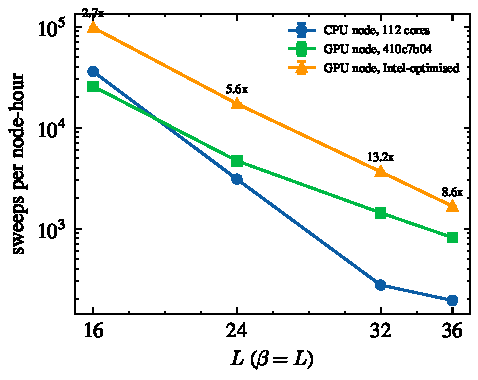
\includegraphics[width=0.6\textwidth]{throughput_vs_L}
\caption{Node throughput of the best layout per side against $L$; the factor is best GPU / best CPU.}
\end{figure}
\begin{figure}[H]\centering
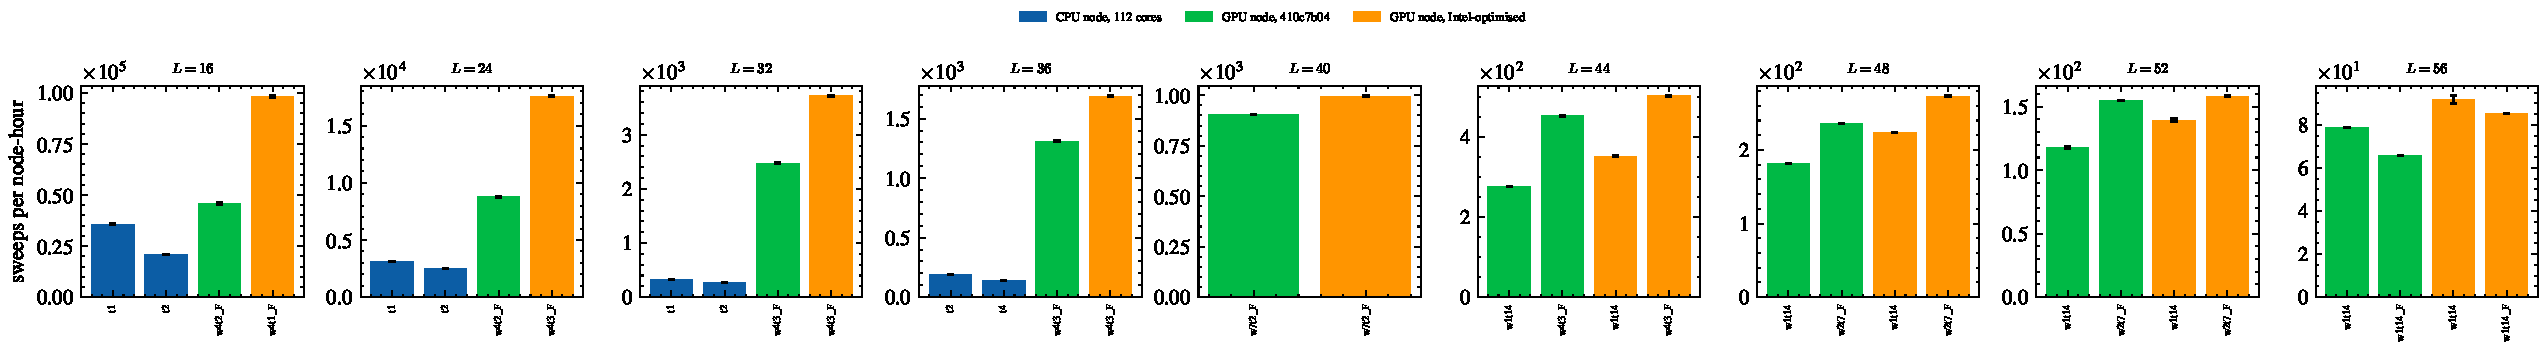
\includegraphics[width=\textwidth]{layout_scan}
\caption{Throughput of every layout (tags as in Tables 1 and 2), one panel per $L$.}
\end{figure}
\begin{figure}[H]\centering
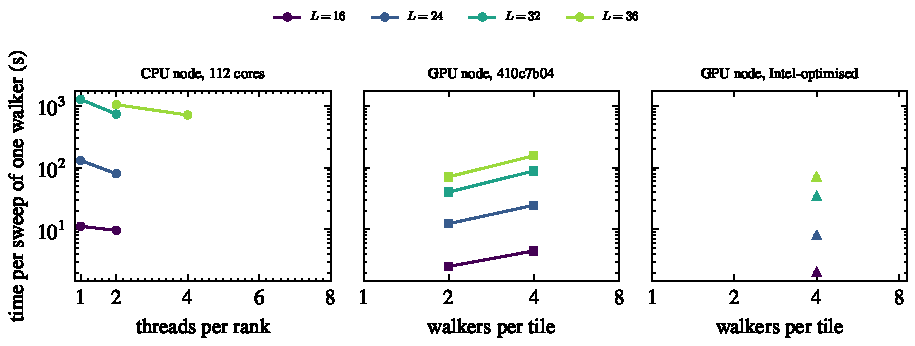
\includegraphics[width=\textwidth]{walker_time}
\caption{Time per sweep of one walker; one panel per side (CPU: against threads per rank, GPU: against walkers per tile), colour = $L$.}
\end{figure}
\begin{figure}[H]\centering
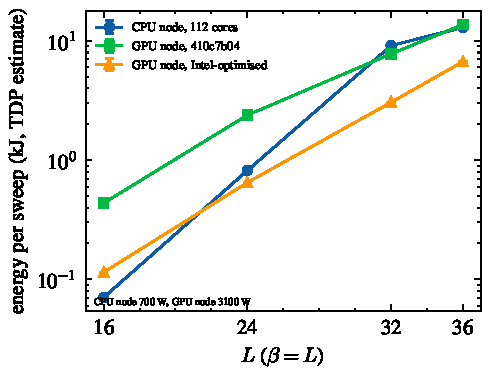
\includegraphics[width=0.6\textwidth]{energy_per_sweep}
\caption{Estimated energy per sweep of the best layout per side.}
\end{figure}
\begin{figure}[H]\centering
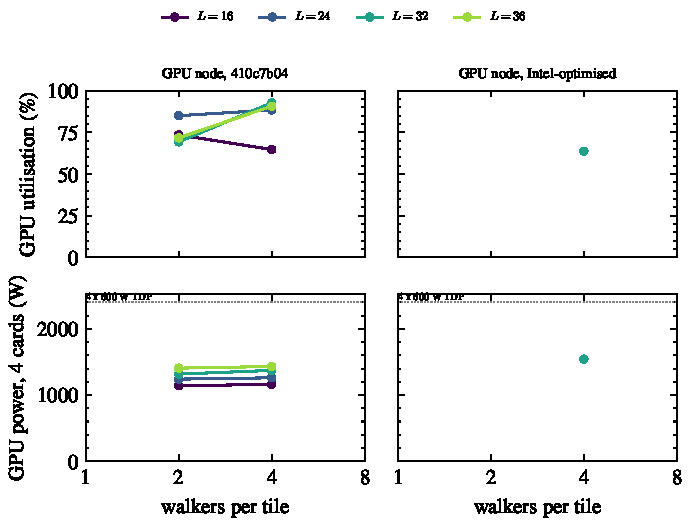
\includegraphics[width=0.7\textwidth]{gpu_usage}
\caption{Mean GPU utilisation (top) and power of the four cards (bottom), xpu-smi 1\,s samples, against walkers per tile; one column per GPU binary, colour = $L$.}
\end{figure}
\end{document}
